\subsection{Integrace do evaluačního procesu}
\label{subsec:implementation-pipeline}

Při odevzdání řešení studentem systém Kelvin spustí evaluační proces zajišťující kompilaci, automatické testy a provedení učitelem vytvořené pipeline.
Souběžně je spuštěn modul LLM analýzy, který ke své práci potřebuje výhradně zdrojové soubory studenta, dostupné ihned po odevzdání.
Paralelní běh je možný proto, že výsledky evaluace nejsou pro LLM analýzu vyžadovány, a zároveň přirozený — výstupy analýzy jsou určeny pouze učiteli a student na ně nečeká, podobně jako u asynchronní kontroly plagiátorství.

Začlenění výsledků evaluace do vstupu LLM analýzy by naopak vyžadovalo sekvenční zpracování a prodloužilo dobu čekání.
Otevřelo by však prostor pro propracovanější analýzu: model by mohl pracovat i s výstupy kompilátoru, například s varováními nebo chybami nástroje Clang, a ve svých návrzích na ně přímo odkazovat.
Toto rozšíření tak představuje přirozený směr dalšího rozvoje implementace.

\begin{figure}[h]
    \centering
    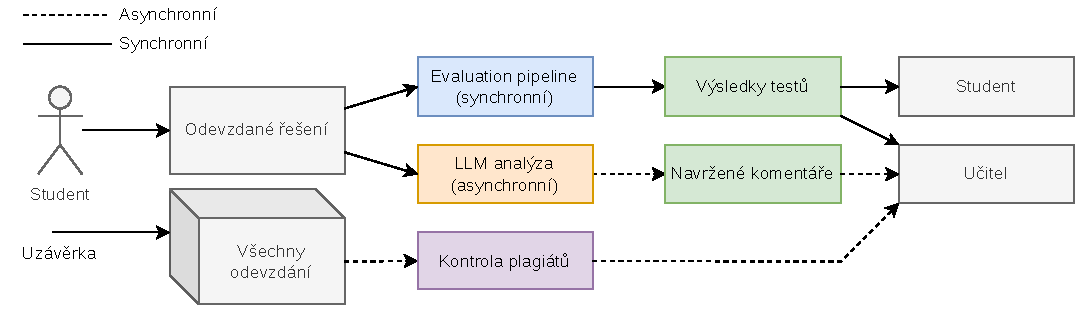
\includegraphics[width=1.0\textwidth]{resources/diagrams/evaluation-pipeline}
    \caption{Zjednodušené schéma zpracování odevzdání v systému Kelvin, znázorňující paralelní běh synchronní evaluační pipeline a asynchronní LLM analýzy}
    \label{fig:implementation-pipeline}
\end{figure}

\endinput